\documentclass[12pt]{article}
\usepackage{amsmath}
\usepackage{subcaption}
\usepackage[utf8]{inputenc}
\usepackage{wrapfig}
\usepackage{float}
\usepackage{graphicx} % Required for inserting images
\usepackage{booktabs} % This and below for tables
\usepackage[breaklinks]{hyperref}
% \hypersetup{colorlinks=true, linkcolor=Black, citecolor=Black, filecolor=Blue,
%     urlcolor=Blue, unicode=true}
\usepackage[margin=1.2in]{geometry} % Adjust border
\usepackage{color}

\renewcommand{\thesubsubsection}{(\alph{subsubsection})}


% For adding R code to appendix
\usepackage[T1]{fontenc}
\usepackage[latin1]{inputenc}

\usepackage{lmodern}% better font than default
\usepackage{tgcursor}% tt font with bold/italic styles

\usepackage{listings}
\lstset{
    language=R,
    basicstyle=\ttfamily
}


\begin{document}


\title{STA4026S Analytics - Neural Networks}

\author{Assignment 1\\
        Laurence Walton\\
        \href{mailto:wltlau003@myuct.ac.za}{wltlau003@myuct.ac.za}
}
\date{August, 2023}

\maketitle
% A
\subsubsection{}
In the context of neural networks the soft-max activation function is used to transform node values from the output layer to values in a probability distribution where each node has a value between 0 and 1 and the sum of the nodes in the layer is 1. This is relevant for multi-class classification problems because with soft-max applied each output node value can be treated as a probability where predictions would correspond to the node with the highest probability. The soft-max function can therefore be seen as an extension of the sigmoid activation function, for multiple classes. The soft-max also ensures that the predictions are scaled such that the relative differences between the predicted probabilities are conserved, which allows for the accurate calculation of the loss (and thus the training of the neural network). If we have \( X \) as an \( N \times p \) matrix (\(N \) training examples, \(p \) features):

\[ X = \begin{bmatrix} 
x_{11} & x_{12} & \ldots & x_{1p} \\ 
x_{21} & x_{22} & \ldots & x_{2p} \\ 
\vdots & \vdots & \ddots & \vdots \\ 
x_{N1} & x_{N2} & \ldots & x_{Np} 
\end{bmatrix} \]

The soft-max of \( X \) (row-wise for each training example) is:

\[ softmax(X) = \begin{bmatrix} 
\frac{\exp(x_{11})}{\sum_{j=1}^{p} \exp(x_{1j})} & \frac{\exp(x_{12})}{\sum_{j=1}^{p} \exp(x_{1j})} & \ldots & \frac{\exp(x_{1p})}{\sum_{j=1}^{p} \exp(x_{1j})} \\ 
\frac{\exp(x_{21})}{\sum_{j=1}^{p} \exp(x_{2j})} & \frac{\exp(x_{22})}{\sum_{j=1}^{p} \exp(x_{2j})} & \ldots & \frac{\exp(x_{2p})}{\sum_{j=1}^{p} \exp(x_{2j})} \\ 
\vdots & \vdots & \ddots & \vdots \\ 
\frac{\exp(x_{N1})}{\sum_{j=1}^{p} \exp(x_{Nj})} & \frac{\exp(x_{N2})}{\sum_{j=1}^{p} \exp(x_{Nj})} & \ldots & \frac{\exp(x_{Np})}{\sum_{j=1}^{p} \exp(x_{Nj})}
\end{bmatrix} \]

\newpage
% B
\subsubsection{}
A potential numerical pitfall in evaluating the cross-entropy error function arises if the predicted probability for a class is 0, as the evaluation would include the logarithm of 0 which is obviously undefined. This is mitigated by using activation functions such as the soft-max, where no predictions can be zero due to exponentiation. However, due to floating point imprecision in software, predictions could be rounded to zero in the soft-max, and therefore cause undefined behaviour in the cross-entropy error function. In the implementation of the soft-max in this assignment, this was avoided by performing the "Log-Sum-Exp" trick, which works by subtracting the maximum value before exponentiation and adding it back after taking the logarithm. This prevents issues related to floating point rounding without altering the actual result.

\begin{figure*}[h]
\centering
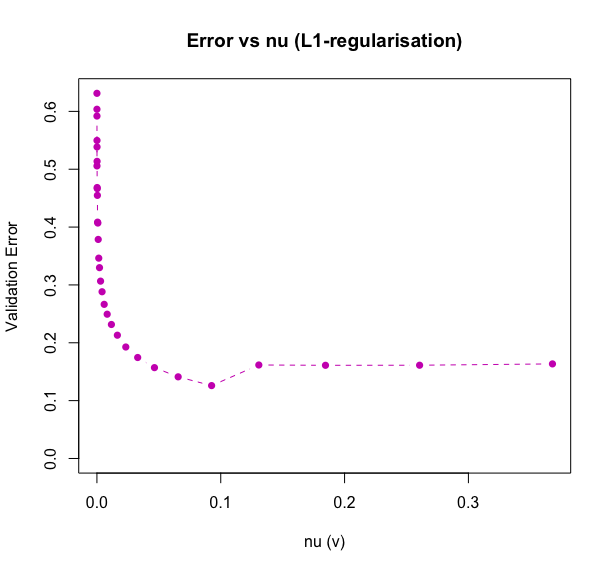
\includegraphics[width=0.8\textwidth]{question_c_plot.png}
\caption{Tanh activations}
\label{fig:fig1}
\end{figure*}

\newpage
% C
\subsubsection{}
Figure~\ref{fig:fig1} shows the cross entropy error obtained on the validation data for varying values of \( \nu \), where I found the \( \nu \) value of \( 0.09261443 \) corresponds to the minimum error of \( 0.1259723 \). Up until the minimum the validation error decreases as the regularisation increases, which is the expected result: we first want our neural network to over-fit the data, and then through regularisation decrease the over-fitting by penalising the complexity of the model. The decreasing validation error shows that as the regularisation increases the model is able to better generalise on unseen data, up until a point where further penalising model complexity just results in worse performance. The regularisation level (value of \( \nu \)) was chosen to be 0.1 for the remainder of the assignment. 


\begin{figure*}[h]
\centering
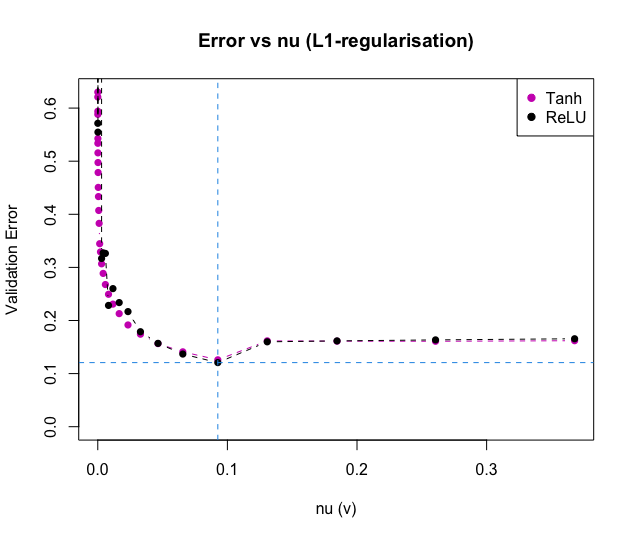
\includegraphics[width=0.8\textwidth]{question_d_plot.png}
\caption{Tanh and ReLU activations}
\label{fig:fig2}
\end{figure*}

% D
\subsubsection{}
Figure~\ref{fig:fig2} shows the previous validation curve but with a new curve also superimposed: that of the same neural network implementation except for the fact that the Rectified Linear Units (ReLU) activation function is used on the hidden layers. For this new validation curve, I found the $\nu$ value of $0.09261443$ corresponds to the minimum error of $0.120692$. This is almost identical to that of the tanh curve, the only difference being the ReLU achieving a slightly lower validation error at the minimum. From the validation plot of these two curves alone, I cannot distinguish a benefit from using either over the other except for this difference, and so would decide to use ReLU over tanh.

\begin{figure*}[h]
\centering
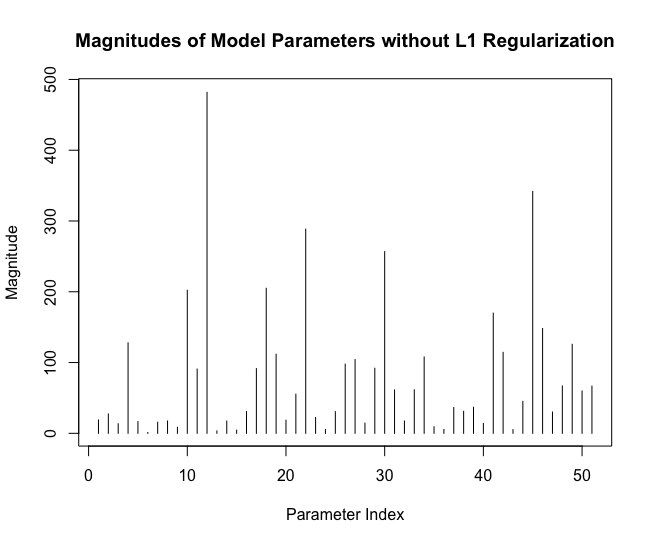
\includegraphics[width=0.6\textwidth]{question_e_plot_B.png}
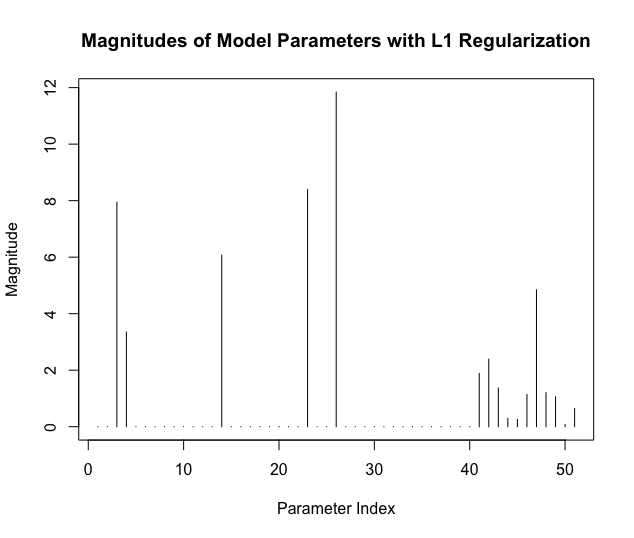
\includegraphics[width=0.6\textwidth]{question_e_plot_A.png}
\caption{Magnitude of model parameters}
\label{fig:fig3}
\end{figure*}

% E
\subsubsection{}
 Figure~\ref{fig:fig3} shows the magnitudes of the ReLU neural network trained on the entire data set, with and without L1 regularization applied. When applied, the regularisation level was set to \( \nu = 0.1 \). Comparing the magnitude of the parameters between these two plots provides insights into the model's complexity. L1 regularization introduces more 'sparsity', essentially reducing the effective number of parameters. In this case specifically, with L1 regularization, many of the model's parameters shrank to near-zero or zero and the largest parameter magnitudes were also reduced. The fact that the regularization promotes such strong sparsity indicates that the original model, without regularization, might have been over fitting the data, capturing too much variance instead of the true underlying patterns. The reduced number of effective parameters show that the model has been able to better capture the underlying pattern and therefore will be able to perform better in its goal of predicting the class of unseen data. This is illustrated in Figure~\ref{fig:fig2} by the decreasing validation error.

% F
\subsubsection{}
From the response curves in Figure~\ref{fig:fig4} it shows that using ReLU activations cause the model to partition the data linearly instead of non-linearly (as seen when using tanh activations). This is to be expected as ReLU is a piece wise linear function that simply outputs the input if it is positive, and zero otherwise. I would argue that in this context the more appropriate choice of activation is the ReLU, as it provides a much simpler and more interpretable rule for making predictions on new bird measurements. We can observe this in the response curve for the ReLU activations: the data is easily separable by two straight lines, forming the three classes in the feature space. This is as opposed to the tanh activations, which has non-linearilty in how it divides the feature space.


\newpage
\appendix
\section{Code}
Raw R code from WLTLAU003\_Analytics\_A1.R:
\newgeometry{margin=0.1in}
\begin{lstlisting}
#
# (a)
#

# Function: softmax_and_log_softmax 
# Description: Apply log of softmax to a matrix (N training examples),
# avoiding over/under flow of values from normal softmax
#
# Arguments:
#   X: A N (no. training examples) x p (no. features) matrix
#
# Returns:
#   1. Matrix of same dimensions as X with softmax applied, 
#   2. Matrix of same dimensions as X with log softmax applied 
#   Done to avoid numerical issues encountered when just taking log
#   of softmax output
softmax_and_log_softmax <- function(X) {
  # Subtracting the max for numerical stability
  max_prob <- apply(X, 1, max)
  X_stable <- sweep(X, 1, max_prob, "-")
  
  # Exponentiating
  exp_X <- exp(X_stable)
  
  # Calculating the sum of exponentials for each row
  sum_exp <- apply(exp_X, 1, sum)
  
  # Calculating softmax
  softmax_X <- sweep(exp_X, 1, sum_exp, "/")
  
  # Calculating log sum of exponentials
  log_sum_exp <- log(sum_exp)
  
  # Calculating log softmax
  log_softmax_X <- sweep(X_stable, 1, log_sum_exp, "-")
  
  return(list(softmax = softmax_X, log_softmax = log_softmax_X))
}


# (b)


# Function: tanh
# Description: Hyperbolic tangent function
tanh = function(z){
  base::tanh(z)
}

# Function: neural_net
# Arguments:
#   X: Input matrix (N x p)
#   Y: Output matrix (N x q)
#   theta: A parameter vector (all of the parameters)
#   nu: Regularisation hyperparameter 
neural_net = function(X, Y, theta, nu)
{
  # Relevant dimensional variables:
  N     = dim(X)[1]
  p     = dim(X)[2]
  q     = dim(Y)[2]
  # Number of nodes (fixed at 8)
  m     = 8
  
  # Populate weight-matrix and bias vectors:
  index = 1:(p*m)
  W1    = matrix(theta[index], p, m) 
  index = max(index)+1:(m*q)
  W2    = matrix(theta[index], m, q)
  index = max(index)+1:(m)
  b1    = matrix(theta[index], m, 1)
  index = max(index)+1:(q)
  b2    = matrix(theta[index], q, 1)
  
  # Updating equations (matrix form)
  # mxN (8x148)
  b1    = matrix(rep(b1, N), nrow=m, ncol=N)
  
  # qxN (3x148)
  b2    = matrix(rep(b2, N), nrow=q, ncol = N)
  
  # pxN (2x148)
  a0    = matrix(t(X), p, N)
  
  # mxN (8x148)   
  a1    = apply(t(W1)%*%a0 +  b1, c(1,2), tanh)
  
  # qxN (3x148)        
  z2    = t(W2)%*%a1 + b2
  
  # Transpose z2 so (148x3)
  z2    = t(z2)
  
  sm    = softmax_and_log_softmax(z2)
  a2    = sm$softmax
  
  # Cross-entropy error function for multi-class problems (q-dim) 
  cross_entropy <- -sum(Y * sm$log_softmax)/N
  
  # Debugging
  if (is.na(cross_entropy)){
    browser()
  }
  
  # Cross-entropy error with L1 penalty applied
  L1 <- cross_entropy + (nu/N * (sum(abs(W1)) + sum(abs(W2))))
  
  # Return predictions and error:
  return(list(out=a2, cross_entropy=cross_entropy, L1=L1))
}


#
# (c)
#

set.seed(2023)

# Read in the data:
dat = read.table('Hawks_Data_2023.txt',h= T)
X   = as.matrix(dat[,4:5], ncol=2) 
Y   = as.matrix(dat[,1:3], ncol = 3)
N   = dim(dat)[1]

# Split data into training and test sets 
set = sample(1:N, 0.5*N, replace=FALSE)
X_train       = matrix(X[set,], ncol=2)
Y_train       = matrix(Y[set,], ncol = 3)

X_validation  = matrix(X[-set,], ncol=2)
Y_validation  = matrix(Y[-set,], ncol = 3)

# Network parameters
p = 2
q = 3
m = 8
npars = p*m+m*q+m+q

seq       = 30
lams      <- exp(seq(-11, -1, length=seq))

# Do the validation analysis in parallel - same idea as using a for 
# loop with the different nu's but in this case they are done 
# in parallel
library(parallel)
validation_error_function <- function(i) {
  nu = lams[i]
  # Return the error with L1 penalty applied when fitting
  obj <- function(pars) {
    res <- neural_net(X_train, Y_train, pars, nu)
    return(res$L1)
  }
  set.seed(2023)
  theta = runif(npars,-1,1)
  res_opt = nlm(obj, theta, iterlim=1000)
  
  res_val = neural_net(X_validation, Y_validation, 
                       res_opt$estimate, 0) 
  return(res_val$cross_entropy)
}
# Number of cores to use (adjust as needed)
num_cores <- detectCores() - 1

# Perform the parallel computation
val_error <- unlist(mclapply(1:seq, validation_error_function, 
                             mc.cores = num_cores))

plot(val_error ~ lams, main = "Error vs nu (L1-regularisation)", 
     type = 'b', pch=16, lty=2, col = 6, lwd = 1, xlab = "nu (ν)", 
     ylab = "Validation Error", ylim=c(0,max(val_error)))

# Vertical line at the value of nu that has minimum val_error
abline(v=lams[which.min(val_error)], col=4, lty=2)
# Horizontal line at minimum val_error
abline(h=min(val_error), col=4, lty=2)
# Minimum validation error
min(val_error)
# Corresponding nu
lams[which.min(val_error)]


#
# (d)
#


# Function: ReLU
# Description: Apply ReLU to a vector (single training example). 
# Uses pmax(z,0) to apply the max-function element-wise
ReLU = function(z){
  pmax(z,0)
}

# Function: neural_net_ReLU
# Description: Identical implementaion as question (b) but with 
# ReLU activation for hidden layer
neural_net_ReLU = function(X, Y, theta, nu)
{
  # Relevant dimensional variables:
  N     = dim(X)[1]
  p     = dim(X)[2]
  q     = dim(Y)[2]
  # Number of nodes (fixed at 8)
  m     = 8
  
  # Populate weight-matrix and bias vectors:
  index = 1:(p*m)
  W1    = matrix(theta[index], p, m) 
  index = max(index)+1:(m*q)
  W2    = matrix(theta[index], m, q)
  index = max(index)+1:(m)
  b1    = matrix(theta[index], m, 1)
  index = max(index)+1:(q)
  b2    = matrix(theta[index], q, 1)
  
  # Updating equations (matrix form)
  # mxN (8x148)
  b1    = matrix(rep(b1, N), nrow=m, ncol=N)
  
  # qxN (3x148)
  b2    = matrix(rep(b2, N), nrow=q, ncol = N)
  
  # pxN (2x148)
  a0    = matrix(t(X), p, N)
  
  # mxN (8x148)   
  a1    = apply(t(W1)%*%a0 +  b1, c(1,2), ReLU)
  
  # qxN (3x148)        
  z2    = t(W2)%*%a1 + b2
  
  # Transpose z2 so (148x3)
  z2    = t(z2)
  
  sm    = softmax_and_log_softmax(z2)
  a2    = sm$softmax
  
  # Cross-entropy error function for multi-class problems (q-dim) 
  cross_entropy <- -sum(Y * sm$log_softmax)/N
  
  # Debugging
  if (is.na(cross_entropy)){
    browser()
  }
  
  # Cross-entropy error with L1 penalty applied
  L1 <- cross_entropy + (nu/N * (sum(abs(W1)) + sum(abs(W2))))
  
  # Return predictions and error:
  return(list(out=a2, cross_entropy=cross_entropy, L1=L1))
}

# Network parameters
p = 2
q = 3
m = 8
npars = p*m+m*q+m+q

seq       = 30
lams      = exp(seq(-11, -1, length.out=seq))

# Do the validation analysis in parallel - same idea as using a for 
# loop with the different nu's but in this case they are done 
# in parallel
library(parallel)
validation_error_function_ReLU <- function(i) {
  nu = lams[i]
  # Return the error with L1 penalty applied when fitting
  obj_ReLU <- function(pars) {
    res <- neural_net_ReLU(X_train, Y_train, pars, nu)
    return(res$L1)
  }
  set.seed(2023)
  theta = runif(npars,-1,1)
  res_opt = nlm(obj_ReLU, theta, iterlim=1000)
  
  res_val_ReLU = neural_net_ReLU(X_validation, Y_validation, 
                                 res_opt$estimate, 0) 
  return(res_val_ReLU$cross_entropy)
}
# Number of cores to use (adjust as needed)
num_cores <- detectCores() - 1

# Perform the parallel computation
val_error_ReLU <- unlist(mclapply(1:seq, 
  validation_error_function_ReLU, mc.cores = num_cores))

# First plot the tanh (pink) line again 
# NOTE: must run loop in prev.question first to obtain val_error 
# Ensure all params the same (ie. iterlim, seq)
plot(val_error ~ lams, main = "Error vs nu (L1-regularisation)", 
     type = 'b', pch=16, lty=2, col = 6, lwd = 1, xlab = "nu (ν)", 
     ylab = "Validation Error", ylim=c(0,max(val_error)))

# Then superimpose the ReLU (black) line
lines(val_error_ReLU ~ lams, type = 'b', pch=16, lty=2, col=9, lwd=1)

# Legend, with Tanh first and then ReLU
legend("topright", col=c(6, 9), legend=c("Tanh", "ReLU"), pch=19)

# Vertical line at the value of nu that has minimum val_error
abline(v=lams[which.min(val_error_ReLU)], col=4, lty=2)

# Horizontal line at minimum val_error
abline(h=min(val_error_ReLU), col=4, lty=2)
# Minimum validation error
min(val_error_ReLU)
# Corresponding nu
lams[which.min(val_error_ReLU)]


#
# (e)
#


# Read in the data:
dat = read.table('Hawks_Data_2023.txt',h= T)
X   = as.matrix(dat[,4:5], ncol=2) 
Y   = as.matrix(dat[,1:3], ncol = 3)
N   = dim(dat)[1]

# Return the error with L1 penalty applied when fitting
obj_full_dataset <- function(pars) {
  res <- neural_net(X, Y, pars, nu)
  return(res$L1)
}


# Return the error with L1 penalty applied when fitting
obj_full_dataset_ReLU <- function(pars) {
  res <- neural_net_ReLU(X, Y, pars, nu)
  return(res$L1)
}

# Network parameters
p = 2
q = 3
m = 8
npars = p*m+m*q+m+q

nu = 0.1
theta   = runif(npars,-1,1)
res_opt = nlm(obj_full_dataset, theta, iterlim=1000)
optimal_pars <- res_opt$estimate

# Plot the magnitudes of the parameters with L1
plot(abs(optimal_pars), type = 'h', xlab = 'Parameter Index', 
     ylab = 'Magnitude', 
     main = 'Magnitudes of Model Parameters with L1 Regularization')

nu = 0
theta   = runif(npars,-1,1)
res_opt = nlm(obj_full_dataset, theta, iterlim=1000)
optimal_pars_no_reg <- res_opt$estimate

# Plot the magnitudes of the parameters without L1
plot(abs(optimal_pars_no_reg), type = 'h', xlab = 'Parameter Index', 
     ylab = 'Magnitude', 
     main = 'Magnitudes of Model Parameters without L1 Regularization')


#
# (f)
#


# Obtain the model trained on the full data set again
# Network parameters
p = 2
q = 3
m = 8
npars = p*m+m*q+m+q
nu    = 0.1
set.seed(2023)
theta   = runif(npars,-1,1)
res_opt = nlm(obj_full_dataset, theta, iterlim=1000)
optimal_pars <- res_opt$estimate

# Construct the plot for response curve
m = 300
wing_dummy       = seq(min(X[, "Wing"]), 
                       max(X[, "Wing"]), 
                       length=m)
weight_dummy     = seq(min(X[, "Weight"]), 
                       max(X[, "Weight"]), 
                       length=m)

plot (1, 1, type = 'n', xlim = range(X[, "Wing"]), 
      ylim = range(X[, "Weight"]),
      xlab="Wing", ylab="Weight")

abline(v=wing_dummy)
abline(h=weight_dummy)
x1 = rep(wing_dummy, m)
x2 = rep(weight_dummy, each=m)
points(x2~x1, pch=16)

# Use points on response curve to create a matrix 
# to be used for getting predictions
X_lattice = data.frame(Wing=x1, Weight=x2)
# The Y values are just zeros - not actually used when making these 
# predicitons as no error is being calculated, just getting the 
# outputs from the NN
m_zeros = rep(0,length=m)
y1 = rep(m_zeros, m)
y2 = rep(m_zeros, m)
y3 = rep(m_zeros, m)
Y_lattice = data.frame(SpecA=y1, SpecB=y2, SpecC=y3)

# Get predictions
res = neural_net(X_lattice, Y_lattice, optimal_pars, 0)
predictions = res$out

# Obtain the class from each prediction by taking the highest 
# probability from softmax output
class = apply(predictions, 1, which.max)
cols = c('blue', 'red', 'lightblue')
plot(x2~x1, pch=16, col=cols[class], xlab="Weight", ylab="Wing", 
     main="Response Curve with Tanh activations")

# Plot the training data with a letter corresponding to the class 
numeric_to_char <- function(x) {
  return(LETTERS[x])
}
labels = apply(Y, 1, which.max)
char_labels = sapply(labels, numeric_to_char)
text(X[, "Weight"]~ X[, "Wing"], labels=char_labels, cex=0.8)



#
# (f) Part 2 (ReLU)
#

# Return the error with L1 penalty applied when fitting
obj_full_dataset_ReLU <- function(pars) {
  res <- neural_net_ReLU(X, Y, pars, nu)
  return(res$L1)
}

# Network parameters
p = 2
q = 3
m = 8
npars = p*m+m*q+m+q
nu    = 0.1
set.seed(2023)
theta   = runif(npars,-1,1)
res_opt = nlm(obj_full_dataset_ReLU, theta, iterlim=1000)
optimal_pars <- res_opt$estimate

# Construct the plot for response curve
m = 300
wing_dummy       = seq(min(X[, "Wing"]), 
                       max(X[, "Wing"]), 
                       length=m)
weight_dummy     = seq(min(X[, "Weight"]), 
                       max(X[, "Weight"]), 
                       length=m)

plot (1, 1, type = 'n', xlim = range(X[, "Wing"]), 
      ylim = range(X[, "Weight"]),
      xlab="Wing", ylab="Weight")

abline(v=wing_dummy)
abline(h=weight_dummy)
x1 = rep(wing_dummy, m)
x2 = rep(weight_dummy, each=m)
points(x2~x1, pch=16)

# Use points on response curve to create a matrix 
# to be used for getting predictions
X_lattice = data.frame(Wing=x1, Weight=x2)
# The Y values are just zeros - not actually used when making these 
# predicitons as no error is being calculated, just getting the 
# outputs from the NN
m_zeros = rep(0,length=m)
y1 = rep(m_zeros, m)
y2 = rep(m_zeros, m)
y3 = rep(m_zeros, m)
Y_lattice = data.frame(SpecA=y1, SpecB=y2, SpecC=y3)

# Get predictions
res = neural_net_ReLU(X_lattice, Y_lattice, optimal_pars, 0)
predictions = res$out

# Obtain the class from each prediction by taking the highest 
# probability from softmax output
class = apply(predictions, 1, which.max)
cols = c('blue', 'red', 'lightblue')
plot(x2~x1, pch=16, col=cols[class], xlab="Weight", 
     ylab="Wing", main="Response Curve with ReLU activations")

# Plot the training data with a letter corresponding to the class 
numeric_to_char <- function(x) {
  return(LETTERS[x])
}
labels = apply(Y, 1, which.max)
char_labels = sapply(labels, numeric_to_char)
text(X[, "Weight"]~ X[, "Wing"], labels=char_labels, cex=0.8)
\end{lstlisting}
\end{document}
